% Options for packages loaded elsewhere
\PassOptionsToPackage{unicode}{hyperref}
\PassOptionsToPackage{hyphens}{url}
\PassOptionsToPackage{dvipsnames,svgnames,x11names}{xcolor}
%
\documentclass[
  letterpaper,
  DIV=11,
  numbers=noendperiod]{scrreprt}

\usepackage{amsmath,amssymb}
\usepackage{iftex}
\ifPDFTeX
  \usepackage[T1]{fontenc}
  \usepackage[utf8]{inputenc}
  \usepackage{textcomp} % provide euro and other symbols
\else % if luatex or xetex
  \usepackage{unicode-math}
  \defaultfontfeatures{Scale=MatchLowercase}
  \defaultfontfeatures[\rmfamily]{Ligatures=TeX,Scale=1}
\fi
\usepackage{lmodern}
\ifPDFTeX\else  
    % xetex/luatex font selection
\fi
% Use upquote if available, for straight quotes in verbatim environments
\IfFileExists{upquote.sty}{\usepackage{upquote}}{}
\IfFileExists{microtype.sty}{% use microtype if available
  \usepackage[]{microtype}
  \UseMicrotypeSet[protrusion]{basicmath} % disable protrusion for tt fonts
}{}
\makeatletter
\@ifundefined{KOMAClassName}{% if non-KOMA class
  \IfFileExists{parskip.sty}{%
    \usepackage{parskip}
  }{% else
    \setlength{\parindent}{0pt}
    \setlength{\parskip}{6pt plus 2pt minus 1pt}}
}{% if KOMA class
  \KOMAoptions{parskip=half}}
\makeatother
\usepackage{xcolor}
\setlength{\emergencystretch}{3em} % prevent overfull lines
\setcounter{secnumdepth}{-\maxdimen} % remove section numbering
% Make \paragraph and \subparagraph free-standing
\makeatletter
\ifx\paragraph\undefined\else
  \let\oldparagraph\paragraph
  \renewcommand{\paragraph}{
    \@ifstar
      \xxxParagraphStar
      \xxxParagraphNoStar
  }
  \newcommand{\xxxParagraphStar}[1]{\oldparagraph*{#1}\mbox{}}
  \newcommand{\xxxParagraphNoStar}[1]{\oldparagraph{#1}\mbox{}}
\fi
\ifx\subparagraph\undefined\else
  \let\oldsubparagraph\subparagraph
  \renewcommand{\subparagraph}{
    \@ifstar
      \xxxSubParagraphStar
      \xxxSubParagraphNoStar
  }
  \newcommand{\xxxSubParagraphStar}[1]{\oldsubparagraph*{#1}\mbox{}}
  \newcommand{\xxxSubParagraphNoStar}[1]{\oldsubparagraph{#1}\mbox{}}
\fi
\makeatother


\providecommand{\tightlist}{%
  \setlength{\itemsep}{0pt}\setlength{\parskip}{0pt}}\usepackage{longtable,booktabs,array}
\usepackage{calc} % for calculating minipage widths
% Correct order of tables after \paragraph or \subparagraph
\usepackage{etoolbox}
\makeatletter
\patchcmd\longtable{\par}{\if@noskipsec\mbox{}\fi\par}{}{}
\makeatother
% Allow footnotes in longtable head/foot
\IfFileExists{footnotehyper.sty}{\usepackage{footnotehyper}}{\usepackage{footnote}}
\makesavenoteenv{longtable}
\usepackage{graphicx}
\makeatletter
\def\maxwidth{\ifdim\Gin@nat@width>\linewidth\linewidth\else\Gin@nat@width\fi}
\def\maxheight{\ifdim\Gin@nat@height>\textheight\textheight\else\Gin@nat@height\fi}
\makeatother
% Scale images if necessary, so that they will not overflow the page
% margins by default, and it is still possible to overwrite the defaults
% using explicit options in \includegraphics[width, height, ...]{}
\setkeys{Gin}{width=\maxwidth,height=\maxheight,keepaspectratio}
% Set default figure placement to htbp
\makeatletter
\def\fps@figure{htbp}
\makeatother

\KOMAoption{captions}{tableheading}
\makeatletter
\@ifpackageloaded{bookmark}{}{\usepackage{bookmark}}
\makeatother
\makeatletter
\@ifpackageloaded{caption}{}{\usepackage{caption}}
\AtBeginDocument{%
\ifdefined\contentsname
  \renewcommand*\contentsname{Table of contents}
\else
  \newcommand\contentsname{Table of contents}
\fi
\ifdefined\listfigurename
  \renewcommand*\listfigurename{List of Figures}
\else
  \newcommand\listfigurename{List of Figures}
\fi
\ifdefined\listtablename
  \renewcommand*\listtablename{List of Tables}
\else
  \newcommand\listtablename{List of Tables}
\fi
\ifdefined\figurename
  \renewcommand*\figurename{Figure}
\else
  \newcommand\figurename{Figure}
\fi
\ifdefined\tablename
  \renewcommand*\tablename{Table}
\else
  \newcommand\tablename{Table}
\fi
}
\@ifpackageloaded{float}{}{\usepackage{float}}
\floatstyle{ruled}
\@ifundefined{c@chapter}{\newfloat{codelisting}{h}{lop}}{\newfloat{codelisting}{h}{lop}[chapter]}
\floatname{codelisting}{Listing}
\newcommand*\listoflistings{\listof{codelisting}{List of Listings}}
\makeatother
\makeatletter
\makeatother
\makeatletter
\@ifpackageloaded{caption}{}{\usepackage{caption}}
\@ifpackageloaded{subcaption}{}{\usepackage{subcaption}}
\makeatother

\ifLuaTeX
  \usepackage{selnolig}  % disable illegal ligatures
\fi
\usepackage{bookmark}

\IfFileExists{xurl.sty}{\usepackage{xurl}}{} % add URL line breaks if available
\urlstyle{same} % disable monospaced font for URLs
\hypersetup{
  pdftitle={Slime Lab Manual},
  pdfauthor={David Bryan},
  colorlinks=true,
  linkcolor={blue},
  filecolor={Maroon},
  citecolor={Blue},
  urlcolor={Blue},
  pdfcreator={LaTeX via pandoc}}


\title{Slime Lab Manual}
\usepackage{etoolbox}
\makeatletter
\providecommand{\subtitle}[1]{% add subtitle to \maketitle
  \apptocmd{\@title}{\par {\large #1 \par}}{}{}
}
\makeatother
\subtitle{(aka fish / wet lab manual)}
\author{David Bryan}
\date{2025-11-20}

\begin{document}
\maketitle

\renewcommand*\contentsname{Table of contents}
{
\hypersetup{linkcolor=}
\setcounter{tocdepth}{2}
\tableofcontents
}

\bookmarksetup{startatroot}

\chapter{Welcome to the Slime Lab}\label{welcome-to-the-slime-lab}

(aka fish / wet lab manual)

\hfill\break

This is the \textbf{Slime Lab Manual}. This document describes
trawl-haul data collection methods, biological sampling requirements,
physical oceanographic measurements, and at sea data processing aboard
the NOAA Ship Oscar Dyson by the Midwater Assessment Conservation
Engineering (MACE) program. Refer to the survey project instructions for
specific information on the primary cruise objectives, basic survey
design, schedule, equipment, gear, Special Studies, etc.

\includegraphics[width=1\textwidth,height=\textheight]{images/age1_pollock.JPG}

\section{How to use this manual}\label{how-to-use-this-manual}

There is a sidebar on the left to navigate to main topics. Within each
topic there is a Table of Contents on the right side of the screen that
can be used to navigate to content within that topic.

\section{Glossary of Terms}\label{glossary-of-terms}

Here is a \hyperref[volun-glossary]{glossary of roles and terms}
relevant to MACE surveys aboard NOAA Ships. This is helpful to anybody
new to the NOAA ship Oscar Dyson.

\section{Quick Links}\label{quick-links}

Here are a few links to some content:

\bookmarksetup{startatroot}

\chapter{Pre-Cruise Preparation}\label{pre-cruise-preparation}

Tasks related to the slime lab that should be completed before boarding
the ship.

\section{A. Equipment Checklist}\label{a.-equipment-checklist}

Gear Inventory (MACE loading and shipping) is a rolling spreadsheet
maintained through Google Sheets to track and inventory gear shipped to
and from Alaska.
\href{https://docs.google.com/spreadsheets/d/12_39Ke-rfvQZLH6ZlejbbX5bNRX2fFNvNkkVWe21Hp8/edit?gid=1672489246\#gid=1672489246}{Click
here to open the Google Sheet}

\section{B. Special Study Supplies}\label{b.-special-study-supplies}

Pre-cruise preparation includes soliciting Special Studies requests for
all surveys during the upcoming year. In November, the MACE Special
Collections Request form is emailed to contacts on the
special\_studies\_announcement\_list which is found in the G:

\special

studies folder under the last survey year. The announcement list is a
living document in which new contacts are added and old or invalid email
addresses are deleted.

After they are received, Special Study requests are put in a subfolder
in G:

\special

studies by year, then by either Winter or Summer. Information should
include 1). project goals with some background information, 2) specific
sampling instructions/procedures which include a) storage requirements,
b) time and space requirements, and c)specific details of any activities
that may impact vessel/MACE personnel or equipment. 3) When and how
supplies, chemicals, and samples will be shipped to and from the vessel,
and 4) a chemical inventory.

\section{C. Sampling Requirements}\label{c.-sampling-requirements}

Obtain information on sampling requirements from stock assessment
authors. Use this to create `Table Tips'.

\section{D. Equipment Calibration}\label{d.-equipment-calibration}

Does it make sense to provide a quick run down of per-cruise
calibrations. i.e.~scales, lenghts boards, SBEs, ect?

\section{E. Age and Growth Supplies}\label{e.-age-and-growth-supplies}

Does organizing the age and growth supplies fall under this manual?

\bookmarksetup{startatroot}

\chapter{Pre-Survey Preparation}\label{pre-survey-preparation}

Tasks to be undertaken prior to leaving the dock. Depending on the
survey some of these tasks may be completed during gear trials.

\section{A. Fish Lab}\label{a.-fish-lab}

\subsection{Equipment}\label{equipment}

If not installed already, under the direction of MACE IT unpack and
connect the \hyperref[length-boards]{length boards} and
\hyperref[marel-scales]{Marel scales} (specimen and basket scales) at
the sampling stations and test the equipment with CLAMS.

While not being used, store and secure the \hyperref[load-cells]{load
cells} in a dry yet accessible location like the ready room. Charge and
store the load cell batteries inside the Chem lab.

During Gear Trials, set up the battery charger in the chem lab and test
both CamTrawl units by deploying them separately on a trawl and
downloading them. For information on CamTrawl setup, download, and
battery charging go to the ``BOC Associated Documents'' folder.

During Gear Trials, do an in-water deployment test with SBE
temperature/pressure data recorder (hereafter, ``SBE'') attached to net
kites, the CamTrawl, and/or survey's CTD. (see section IV.A. - SBE 39
Temperature/Pressure data recorder instructions).

The SBE 39 plus manual is located in the ``BOC Associated Documents''
folder. ( I can not find this)

After you've set up the fish lab (generally, during gear trials or at
the start of the summer survey), test out all the scales, length boards,
and CLAMS stations. The safest way to do this is to confirm with MACE IT
that the CLAMS active survey is `SS Fake Ship'- this ensures that test
data doesn't contaminate real survey data. Check with the IT staff to
set this up. Once you have set the CLAMS survey to SS Fake Ship, go
through a simulated haul in the fish lab (see details on standard haul
processing tasks below) remember to check all protocols are correct for
this survey including any additional protocol needs from Special Studies
(fin clips, stomachs etc.).

\subsection{Cheat Sheets}\label{cheat-sheets}

\begin{itemize}
\tightlist
\item
  Post Table Tips in the fish lab on inboard wall near work station 1.
\item
  Post Special Studies summaries and specific instructions and prepare
  any necessary.
\item
  Post the large MACE ID poster on the wall nearest the ready room.
\item
  Post maturity code descriptions on wall near CLAMS station 4.
\end{itemize}

\subsection{Other Gear}\label{other-gear}

\begin{itemize}
\tightlist
\item
  Set out and arrange fish lab gloves, nitrile gloves, work gloves, and
  staff raingear in the ready room area.
\item
  Set out otolith vials/caps, scalpels, tweezers, knives, pencils in a
  tub next to sink in fish lab.
\item
  Prepare oto juice - (instructions??)
\end{itemize}

\section{B. Chem Lab}\label{b.-chem-lab}

\begin{itemize}
\tightlist
\item
  Set out essential waterproof identification books and laminated id
  cheat sheets (e.g.~myctophid and jellyfish) in a location in the chem
  lab that is easily accessible.
\item
  Unpack totes of office supplies and excess fish lab sampling tools
  into drawers. Organize and label drawers by supply type for ease of
  access (e.g.~Office Supplies, Fish Lab, Bags, Tapes and Bungees etc.).
\end{itemize}

\section{C. Otoliths}\label{c.-otoliths}

Prepare Otolith supplies: Affix enough barcode labels to vials to fill
2-3 boxes. Labeled vials are arranged Left to Right, Top to Bottom (No
Zigzag) in Styrofoam trays. Write the cruise info using permanent marker
on the otolith boxes: (i.e.~- DY2401 where DY = ship name Dyson, 24 =
last 2 digits of year, 01 = cruise \#), vial barcode \# range, and the
species collected.

\section{Length Boards}\label{length-boards}

If lengths are not measuring correctly you may need to re-calibrate the
fish length boards (caution, the ruler inlayed on the length board is
not a precise measuring tool and not used for calibration): * Place the
magnet over the clear plexiglass plate right above the green led light.
The light should turn red and then the length board should switch to
calibration mode. * The screen on the length board will display
calibration mode and it will instruct you to place the magnet at 0 cm of
the metric ruler (This should be up against the vertical barrier between
the plexiglass covered control panel and the inlayed ruler). * The
screen will then instruct you to place the magnet at 75 cm of the metric
ruler (not the ruler inlayed). The 75 cm mark is noted (in permanent
ink) on each fish board. The calibration mode will then finish and let
you know when calibration is complete.

\section{Weighing Scales}\label{marel-scales}

Locate the scale calibration weight sets in the Chem lab floor cabinet
aft of the computers and complete a full calibration test.

See section II -- ``Scale Calibration Marel M1100'' for full calibration
procedures. The full calibration test is separate from the scale
calibration that should be done at the start of each haul (see below).
The test weights for the full calibration should remain stored in a dry
secure location after use. The full scale calibration results should be
documented in on the full scale calibration test sheet which is found in
the current year's MACE loading and shipping google sheet. Copy and
paste the link below in a browser or ask MACE staff to share access to
the latest gear inventory link (Permission may be required to access).

\section{Load Cells}\label{load-cells}

Compare the crane scale readouts to the load cell weights. Have both
cranes (starboard and port) lift an object on the back deck. This could
be a codend or any gear. The weight read out will display in the wet lab
by clams station 1 and on the crane. Attach the loadcell and weigh the
same object, compare for accuracy. If the crane weights are not similar
to the loadcell do not use the crane readouts for fishing operations.
See section Splitter Bin Vs. Sorting Table? for safely using the
loadcell during fishing operations.

\bookmarksetup{startatroot}

\chapter{Pre-Haul Preparation}\label{pre-haul-preparation}

It is the responsibility of the Chief Scientist or their designee to
determine the areas/depths where trawl hauls will be made. Decisions
will be based on a semi-systematic, opportunistic sampling scheme to
maximize the value of each sample with respect to the objectives of the
survey. Once the timing of sampling has been determined there are
several items that can be prepared in the fish lab.

\section{SBE}\label{sbe}

When ``Fishing, Fishing, Fishing'' has been called and/or the net is
being setup on deck, initiate the SBE at least 15 minutes prior to
fishing (see section IV.A. - SBE 39 Temperature/Pressure data recorder
instructions). Your presence may be requested on the bridge for the 15
minute whale watch, so do this before you head up to the bridge.

\section{CamTrawl}\label{camtrawl}

Ensure a charged CamTrawl battery is placed in the CamTrawl, connected,
closed, and secured with ``spaghetti'' locking cord. Verify that the
green light is slowly blinking on the dummy plug before deck crew
attaches the assembly to the net. Floats should be upright or to the
port side if laying down on top of the net The deck crew is responsible
for securing the CamTrawl to the net. See G:\Book of the CAVE and
SOPs\BOC\BOC Associated Documents\CamTrawl for the latest CamTrawl quick
guide.

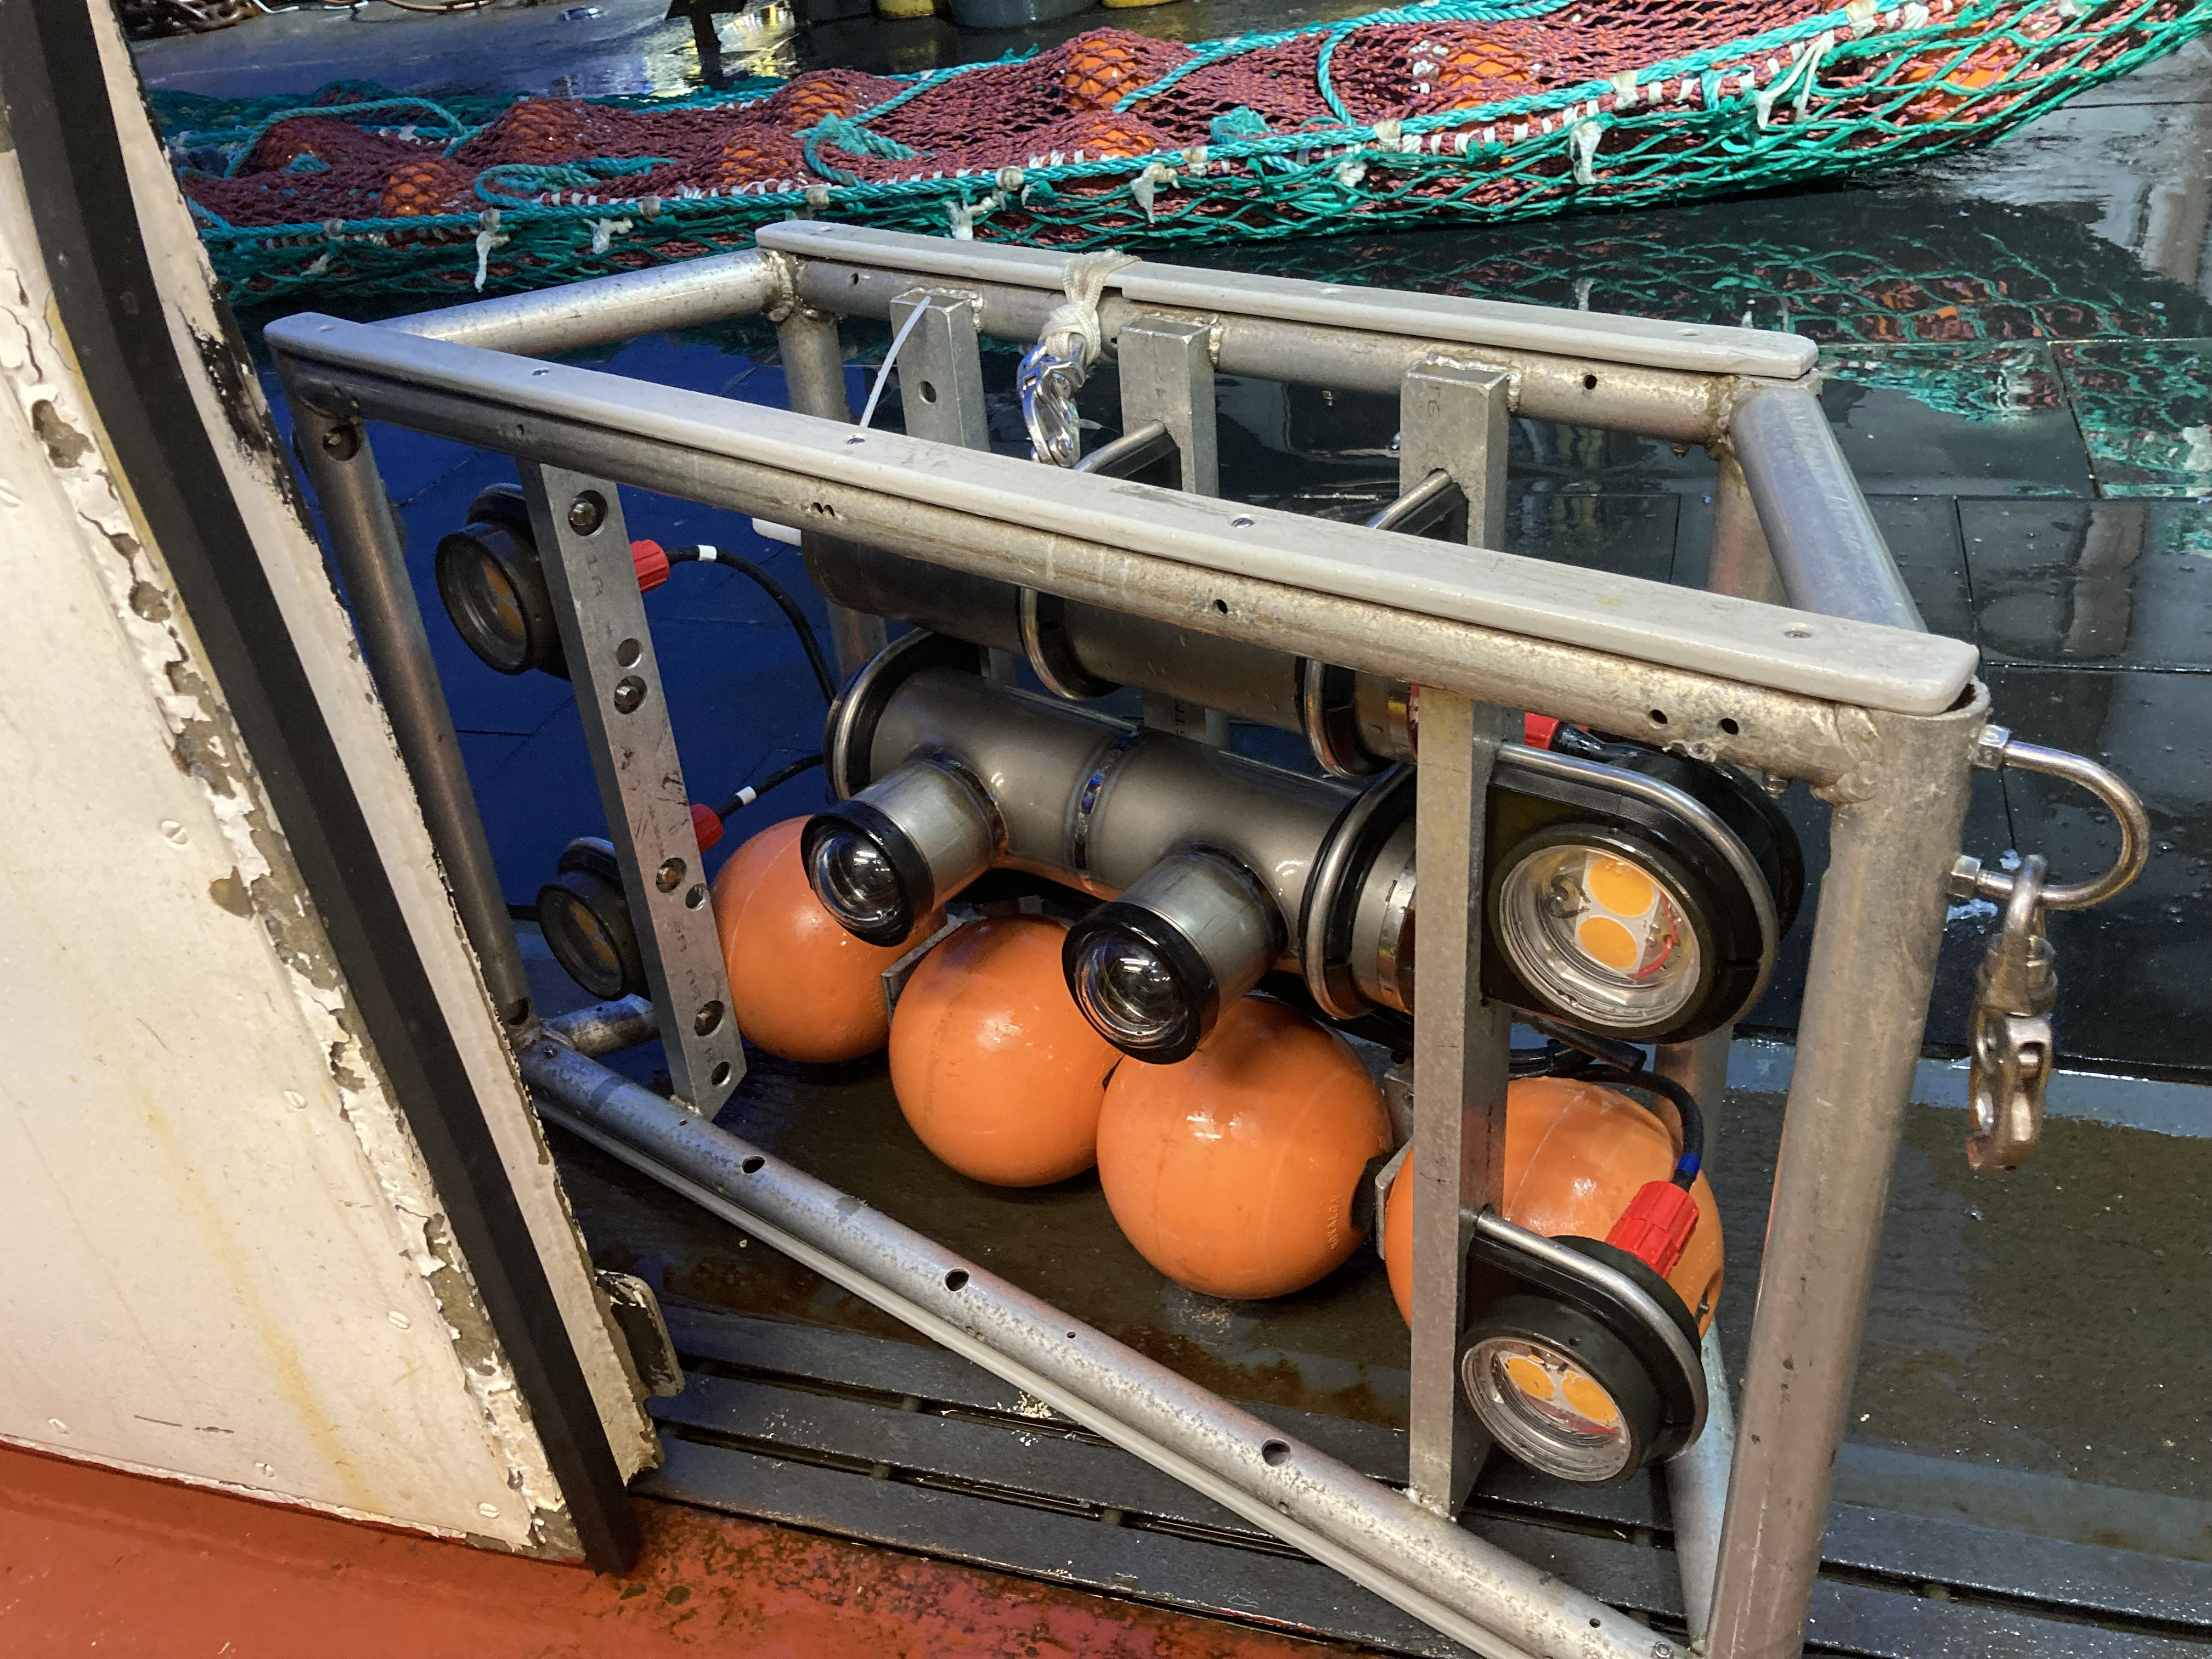
\includegraphics[width=1\textwidth,height=\textheight]{images/camtrawl.jpg}

\section{Marel Scales}\label{marel-scales-1}

The large basket scale (at the end of the conveyor belt) and the smaller
specimen scales (on the counters) require calibration before each haul
is processed - use the stainless steel 20 kg (large scale) and 2 kg
(small scale) weights provided for this purpose for each scale
respectively. Remove all objects from scale and dump any water collected
on top the 20 kg weight.

\textbf{Marel M1100 Calibration:}

\begin{enumerate}
\def\labelenumi{\arabic{enumi}.}
\tightlist
\item
  Simultaneously press the MENU and ZERO keys:
\end{enumerate}

\begin{itemize}
\tightlist
\item
  Wait until the scale asks for a reference weight -- May take 15
  seconds. ``Put 20'' or ``Put 2'' will display.
\end{itemize}

\begin{enumerate}
\def\labelenumi{\arabic{enumi}.}
\setcounter{enumi}{1}
\tightlist
\item
  Place the reference weight (i.e.~20 or 2 kg weight) on the platform
  then press the PRINT key:
\end{enumerate}

\begin{itemize}
\tightlist
\item
  The message ``==='' appears on the display while the calibration takes
  place.
\item
  When the calibration is complete, the message ``Fit nn'' appears.
\item
  Values above 25 indicate a poor calibration; repeat calibration if
  needed.
\end{itemize}

\textbf{Notes:}

\begin{itemize}
\tightlist
\item
  While using the scale, Grade should be selected not Packing. Use the
  up or down arrow to change. The scale will not input weight into Clams
  when in Packing mode.
\item
  Place an empty basket or tub on the scale and press ``Tare''. You are
  ready to weigh baskets!
\item
  If the scale is not steady and it has become more difficult to collect
  weights it may be necessary to recalibrate scales particularly if
  weather changes or the ride of the ship changes between the initial
  calibration and getting back on transect.
\end{itemize}

\section{Other Items}\label{other-items}

Replace and refill standard sampling supplies such as scalpel blades,
the glycerol thymol squeeze bottle, vials caps, and the otolith vials
trays as needed.

Determine if special study requests are applicable for the region and
haul type and prepare for sampling if necessary (i.e., set up supplies,
prepare labels, ovary bags, storage bags).

\includegraphics[width=1\textwidth,height=\textheight]{images/orcas.jpg}

\section{Protected Species Watch (AKA Whale
Watch)}\label{protected-species-watch-aka-whale-watch}

Check in the with FPC or Cave Lead to determine if you are requested to
complete a whale watch on the bridge 15 minutes prior to the net
entering the water. Updated protocols for protected species observation
and avoidance measures is located in the ``BOC Associated Documents''
folder or the current cruise folder. For 2025, look for the document
titled ``MACE protected species at-sea procs\_FY25\_v11.docx''. When
beginning whale watch a common practice is to check in with the Officer
on Deck (OOD) and ask if they have seen any protected species near the
fishing location and what direction the ship will be heading for
fishing, therefore to focus observation in that direction.

\bookmarksetup{startatroot}

\chapter{Sampling Procedures}\label{sampling-procedures}

\section{Saftey and Ergonomics}\label{saftey-and-ergonomics}

Prior to beginning sampling, take time to consider physical saftey and
ergonomics. There are several steps that can be taken.

\begin{itemize}
\tightlist
\item
  Consider some pre sampling stretches to warm up muscles (link to GAP
  stretches).
\item
  The fish lab is wet and slippery, make sure that the non-slip floor
  mats are placed at all workstations.
\item
  Remember to limit basket weights to 20 kg to prevent injuries and
  practice safe \hyperref[lifting]{lifting techniques}.
\item
  use two people to move heavy objects like the camtrawl or large totes
  of fish from the deck.
\end{itemize}

\section{Midwater or Bottom Trawl
catches}\label{midwater-or-bottom-trawl-catches}

\subsection{1. Recording the catch in
CLAMS}\label{recording-the-catch-in-clams}

Open the Catch Logger for Acoustic Midwater Surveys (CLAMS) app; See the
document CLAM Digging located in the folder G:\CLAMS for entering catch
data on the CLAMS app. See the latest power point document
``\ldots Table Tips'' for specific survey sampling guidelines, found in
the cruise folder or posted in the fish lab

\subsection{2. Equipment Retrieval}\label{equipment-retrieval}

As the net is hauled back, obtain the SBE (see section IV.A. - SBE 39
Temperature/Pressure data Midwater recorder instructions) from the deck
crew and download it as soon as possible. The SBE downloader app is
located on the forward computer nearest the sink. Follow the protocols.

Rinse the CamTrawl with fresh water and if time allows download the
images before the next deployment. For information on CamTrawl
deployment and downloading go to the ``BOC Associated Documents''
folder. Staff should familiarize themselves with the ``Camtrawl quick
guide'' procedures just in case. However, MACE IT will most often
download the CamTrawl images after the haul has been processed.

It is common for other equipment to be handed over to the slime lab from
the deck crew; various integrated trawl instrumentation (ITI) and
special study instrumentation (light sensors, etc.).

\subsection{3. Splitter Bin Versus Sorting
Table}\label{splitter-bin-versus-sorting-table}

Catches with a total catch weight of less than \textasciitilde{} 2,000
kg (2 tons) can be dumped directly into the sorting table (link to that
section) However, for larger catches (\textgreater2,000 kg) they must
first go into a deck ``splitter'' bin and are ``split'' for a subsample.

\subsection{Splitter Bin}\label{splitter-bin}

\begin{itemize}
\item
  For split catches, a total catch weight must be obtained by weighing
  the catch in the codend. The load cell(provide link to instructions)
  or the crane scale may be used. Each (?) crane has an internal scale
  that has a readout both at the crane and in the fish lab. However the
  crane scales and/or the readout in the fish lab is not always
  reliable. A weight from the load cell is preferred.
\item
  Once the load cell is secure and hanging from the crane hook press
  TARE and you are ready to weigh the codend.
\item
  After the codend is weighed and recorded the catch is dumped into the
  deck ``splitter'' bin.
\item
  Next the the weight of the empty codend should be recorded.
\item
  A cargo (brailer) net attached to a metal frame in the bottom of the
  splitter bin is used to collect a subsample of the catch. This
  subsample is then lifted into the sorting table.
\item
  Once the crane is secure, wear PPE and receive deck permission to
  check the sorting table and splitter bin to make sure the catch is
  representative/homogenous.
\item
  The total catch weight is the difference of the full codend and the
  weight of the empty codend. The load cell can output in either pounds
  or kilograms. Make sure the load cell reads in kilograms, otherwise
  select the pounds unit in CLAMS.
\end{itemize}

\textbf{Splitter Tips}

\begin{itemize}
\item
  If getting weights from the load cell on deck, checking the splitter
  bin, or checking the sorting table make sure you are wearing PPE
  (helmet + floatation, either a float coat or life jacket)! Also make
  sure the deck crew know you are out there.
\item
  Deleted a not about using Whole Haul here. I think the practice of
  doing that is discouraged. maybe want to double check that whole haul
  sampling for a single species is described somewhere for example in
  case of a shark.
\item
  If the total catch exceeds the capacity of the deck ``splitter'' bin
  and the catch is not homogenous, splits should be repeated (with
  subsequent emptying of the bin) until the entire codend is empty.
  Alternately, the end of the codend has been pinched off at the thick
  strap and placed into the sorting table and the rest of the catch
  dumped overboard. This is not ideal but has happened due to excessive
  catch, poor weather conditions, and inexperienced crew preventing safe
  splitter bin operations.
\end{itemize}

\section{Slime Line}\label{slime-line}

The catch from the sorting table flows directly onto the `slime line'
though a hydraulic door.

\section{Lifting techniques}\label{lifting}

OSHA Proper Lifting Techniques: Safe Lifting Ergonomics
https://www.osha.com/blog/proper-lifting-techniques

Safe lifting involves:

\begin{itemize}
\tightlist
\item
  Standing as close to the load as possible
\item
  Planting your feet shoulder-width apart with one foot slightly ahead
  of the other
\item
  Bending at the hips and knees only until you're deep in a squatting
  position
\item
  Keeping your head up and straight with your shoulders back to keep
  your back straight
\item
  Holding the load close to your body at waist height
\item
  Engaging your core muscles as you push against the ground and
  straighten your legs
\end{itemize}

Here are a few essential don'ts to keep in mind for good lifting
ergonomics:

\begin{itemize}
\tightlist
\item
  Never twist your torso while lifting. Stay ``nose between your toes.''
\item
  Never lift a heavy item above shoulder level.
\item
  Never carry a load that obstructs your vision.
\item
  Never hold your breath while lifting, moving, and setting the load
  down.
\end{itemize}

As you carry the load to its destination, you want to maintain good
ergonomics. That means:

\begin{itemize}
\tightlist
\item
  Holding the load as close to your body as possible, level with your
  belly button
\item
  Keeping your shoulders in line with your hips as you move -- don't
  twist your trunk
\item
  Changing direction with your feet and leading with your hips
\item
  Taking small steps and keeping a good grip with all your fingers
\end{itemize}

Setting down a heavy object is just as dangerous as picking it up.
You'll want to reverse the lifting process, following the same ergonomic
lifting principles:

\begin{itemize}
\tightlist
\item
  Keep the load close to your body and your back straight or slightly
  arched
\item
  Squat down, bending only at the knees and hips
\item
  Tighten your stomach muscles (engage your core) as you lower yourself
\item
  Kneel on one knee if necessary
\end{itemize}

\bookmarksetup{startatroot}

\chapter{}\label{section}

\bookmarksetup{startatroot}

\chapter{}\label{section-1}

\bookmarksetup{startatroot}

\chapter{Volunteer Glossary}\label{volun-glossary}

Glossary of Roles and Terms Relevant to MACE surveys aboard NOAA Ships A
non-exhaustive list of people, places and things relevant to surveys on
the NOAA ship Oscar Dyson.

\subsection{People}\label{people}

\textbf{NOAA Corps} - Commissioned Officer Corps, one of eight federal
uniformed services of the United States, and operates under the National
Oceanic and Atmospheric Administration. Always dressed in navy blue when
at sea. Serve \textasciitilde2 year billets alternately at sea or land
based assignments.

\begin{itemize}
\tightlist
\item
  \textbf{CO}- Commanding Officer, captain of the ship and person
  responsible for all matters pertaining to safety, management,
  operations, and physical condition of the ship and makes the final
  call on all decisions affecting the ship and crew
\item
  \textbf{XO}- Executive Officer, second in command after the CO.
  Responsible for resource management by overseeing ship personnel,
  materials, and budget.
\item
  \textbf{Ops}- Operations Officer, Serves as liaison between science
  party and CO and thus serves as the primary point of contact between
  the science party and ship, coordinates day to day operations between
  the science party and ship.
\item
  \textbf{Nav}- Navigations Officer, in charge of safe navigation and
  completion of appropriate route planning
\item
  \textbf{Ensign}- Junior officer, relatively new to the ship and has
  limited survey experience
\item
  \textbf{MPIC}- Medical Person In Charge, a member of the NOAA corps
  with extra medical training who can provide seasickness meds and who
  can consult a physician on call to provide other medication if needed.
\item
  \textbf{OOD}- Officer on Duty/Deck, an Officer who is in charge of the
  ship for the day or watch
\end{itemize}

\textbf{Civilian crew} - non-commissioned civilian crew members that are
either ``permanently'' assigned to the ship or are in the augment
(rotational) pool for NOAA ships.

\begin{itemize}
\tightlist
\item
  \textbf{Chief Stew(ard)}- Head cook, Prepares menu and meals and
  ensures provisions are secured for surveys. Stationed in the galley,
  good person to know and be in good rapport with! Oversees the Steward
  or 2nd Cook.
\item
  \textbf{2nd Cook} - Assists Chief Steward!
\item
  \textbf{Chief Engineer} - Lead engineer, in charge of all the moving
  parts of the ship that aren't nets. Oversees the 1st Engineer, 2nd
  Engineer, 3rd Engineer, and General Vessel Assistant (GVA, or
  ``Wiper'').
\item
  \textbf{Chief ET} - Ship's electronics technician responsible for
  keeping all the ship's computers and electronic equipment functioning.
  The person that connects personal devices to the ship's Wi-Fi and
  keeps us connected to the rest of the world when at sea.
\item
  \textbf{Chief Boatswain (Bo'sun)}- In charge of fishing and deck
  operations including any over the side activities (CTD's, small boat
  deployments and usage, mooring deployments, etc.), almost always leads
  fishing operations during the day. With Lead Fishermen, oversees the
  Deck Crew.
\item
  \textbf{Lead Fisherman} - Leads fishing ops during the 2nd shift,
  second in charge of deck operations after the Bo'sun, not the same
  person as the Chief Bo'sun! With the Chief Bo'sun, oversees the Deck
  Crew. Senior Survey Tech- Maintains the scientific seawater sampling
  system and other tools used during fishing operations. Survey techs
  also help during trawling and over the side operations. In charge of
  verifying cleanliness of wet lab at end of survey. Oversees the Survey
  Tech.
\end{itemize}

\textbf{Science crew} - civilian NOAA employees (primarily) in charge of
the scientific operations.

\begin{itemize}
\tightlist
\item
  \textbf{Chief Scientist (CS) or Field Party Chief (FPC)} - Science
  leader, in charge of science decision-making during this survey.
\item
  \textbf{Night cave} - Science lead from 4pm to 4am, makes fishing and
  survey-related choices and assists the FPC.
\item
  \textbf{Wet lab leads} - Day and night wet lab leads are in charge of
  fish processing and setting up the camtrawl and the SBE prior to
  trawling. They're situated in the chem lab when not processing fish in
  the wet lab.
\item
  \textbf{ET/IT} - MACE's electronics and software tech. Troubleshoots
  problems with the echosounder, CLAMs, and MACE's analysis software.
\end{itemize}

\subsection{Specific places}\label{specific-places}

\begin{itemize}
\tightlist
\item
  \textbf{Flying Bridge}- Located outside, atop the bridge. Many of the
  officers want people to ask permission to spend time up here. Even if
  they don't, it's a good idea to tell someone you're going up. Bridge-
  This is the uppermost interior deck, immediately below the flying
  bridge. This is the place where the ship's navigation, steering, and
  trawling operations take place. Nobody calls the bridge the 03 deck,
  even though that seems like it makes sense. You are welcome to visit
  the Bridge, except when the ship is leaving the dock or docking, or if
  you are asked to leave.
\item
  \textbf{02 (oh-two) deck}- The deck where the CO, XO, some of the
  other officers, and the Chief Scientist have their staterooms. Also
  where the hospital and XO's office are located. Up one ladder (stairs
  on ships are called ladders!) from the 01 deck.
\item
  \textbf{01 (oh-one) deck}- The deck where the science staterooms and
  the lounge are.
\item
  \textbf{Main deck}- Where the Fish Lab, Chem Lab, and Acoustics Lab
  (or ``Cave'') are located. This could be called the 1 deck.
\item
  \textbf{Mess Deck}- This is where the crew eat, not to be confused
  with\ldots{}
\item
  \textbf{Galley}- This is where the stewards do the cooking.
\item
  \textbf{Fish Lab- Aka wet lab}- location where we in MACE process the
  catch
\item
  \textbf{Chem Lab} - Adjacent to the fish lab, has two MACE computers
  set up, chemicals are stored there and there's a hood in there also.
\item
  \textbf{Cave- Aka the Acoustics Lab}- this is where the MACE science
  team monitors the acoustics and makes decisions about trawling. We
  also work with the incoming data from here. It's where you'll find the
  Chief Scientist, Night Cave, and ET/IT unless they are fishing,
  eating, or sleeping.
\item
  \textbf{Hero Deck aka Side Sampling Station or Ops Deck}- located
  outside on the starboard side of the Chem Lab, this is where ``side
  ops'' are done. When we lower something that isn't a trawl over the
  side of the ship, it goes in the water here. 2 deck- The deck below
  the main deck where crew staterooms, laundry, the gyms, and the engine
  room are all located.
\item
  \textbf{Forward gym}- small gym where treadmill, some weights, and
  rowing machine are located.
\item
  \textbf{Aft gym- aka iron gym}- shares space with the wire room where
  the huge winches that operate the trawls are located. This gym has
  more weights, and it is very loud down there while fishing operations
  are happening.
\item
  \textbf{Laundry room}- located down the ladderwell just forward of the
  starboard forward hatch in the mess deck.
\end{itemize}

\subsection{General places}\label{general-places}

\begin{itemize}
\tightlist
\item
  \textbf{Trawl alley and trawl ramp}- At the back (aft) of the ship,
  where the trawl is deployed.
\item
  \textbf{Ladderway}- Stairs on a ship.
\item
  \textbf{Passageway}- Hallway on a ship.
\item
  \textbf{Gangway}- Mobile bridge used to embark and debark the vessel.
\item
  \textbf{Head}- bathroom on a ship.
\item
  \textbf{Weather deck/decks} - Decks that are open to weather, often
  secured during heavy seas/heavy freezing spray/other extreme weather
  conditions.
\item
  \textbf{Port/Starboard} - Port is the left side when you're facing the
  bow (the pointy end in front) of the ship, and starboard is the right
  side. These terms help mariners avoid confusion about left \& right,
  because they remain fixed regardless of which way the mariner faces.
\item
  \textbf{Stern}- Back end of a ship.
\end{itemize}

\subsection{Things you might hear (and what they
mean)}\label{things-you-might-hear-and-what-they-mean}

\begin{itemize}
\tightlist
\item
  \textbf{``All stations''}- An announcement that pertains to everyone-
  listen up!
\item
  \textbf{``Secure the laundry''}- Don't use the laundry.
\item
  \textbf{``Secure the water''} - You probably get this by now.
\item
  \textbf{``Stand-by''}- Wait. Something might be happening.
\item
  \textbf{``This is a drill, this is a drill''} - Clearly, this is a
  drill, but what kind of drill?!? If you listen(ed) during the welcome
  aboard briefing, you'll know that there are three kinds of drills;
  Ffire, Spill, MOB, Abandon Ship.
\item
  \textbf{``Dog all doors/dogs''}- This is referring to the metal
  latches on the inside of the doors that lead out to weather decks.
  They keep the doors closed and make it so the watertight seals
  function. Sadly, there are no actual dogs aboard ship.
\end{itemize}

\subsection{Gear}\label{gear}

\begin{itemize}
\tightlist
\item
  \textbf{SBE- aka ``pipe bomb''}- Sea Bird Electronics instrument used
  to measure the pressure/temp/salinity/depth that we place on the head
  rope of trawl nets. Yes, it's a terrible nickname.
\item
  \textbf{CTD}- Conductivity, Temperature, Depth instrument that's
  deployed from the Hero Deck. Sometimes referred to as the CTD rosette.
\item
  \textbf{LFS-trawl/net}- This is the main midwater fishing net that
  MACE uses to sample the fish population, it works in tandem with
  the\ldots{}
\item
  \textbf{PNE} - ``Poly Nor'Eastern'' net used for fishing on bottom. Is
  smaller than the midwater net and has roller gear on the footrope.
\item
  \textbf{83-112}- A second kind of bottom- trawl net with roller gear.
  Methot- Square-frame net designed to sample krill and other large
  zooplankton. Deployed via the trawl ramp but uses a different winch.
\item
  \textbf{Centerboard}- Extends
\item
  \textbf{Transducers aka 'ducers or echosounders}- 18, 38, 70, 120,
  200, and 330 kHz acoustic transducers that are mounted on the bottom
  of the ship's centerboard and send active sound waves (pings) towards
  the bottom of the ocean.
\item
  \textbf{Camtrawl}- the camera system that we attach to the LFS trawl.
  It is a stereo camera, which means we can get fish lengths from it. It
  also lets us know where fish are in the water column.
\end{itemize}




\end{document}
